\documentclass[11pt]{article}

\usepackage{amsmath,amssymb}
\usepackage{amsthm}
\usepackage{graphicx}
\usepackage{booktabs}
\usepackage{hyperref}
\usepackage{geometry}
\usepackage{algorithm}
\usepackage{algpseudocode}
\usepackage{caption}
\usepackage{subcaption}
\usepackage{tikz}
\usepackage{pgfplots}
\usepackage{placeins}
\usepackage{float}
\pgfplotsset{compat=1.18}
\usetikzlibrary{positioning,arrows.meta,patterns,calc,decorations.pathreplacing}

\geometry{margin=1in}

% Theorem environments
\newtheorem{theorem}{Theorem}
\newtheorem{lemma}[theorem]{Lemma}
\newtheorem{corollary}[theorem]{Corollary}
\newtheorem{proposition}[theorem]{Proposition}
\theoremstyle{definition}
\newtheorem{definition}[theorem]{Definition}
\newtheorem{example}[theorem]{Example}
\theoremstyle{remark}
\newtheorem{remark}[theorem]{Remark}

\title{DeltaSort: Incremental repair of sorted arrays with known updates}
\author{Shubham Dwivedi \\
\small Independent Researcher \\
\small \texttt{shubd3@gmail.com}
}
\date{January 2026}

\begin{document}
\maketitle

\begin{abstract}
Maintaining sorted order under incremental updates is a common requirement in read-heavy systems,
yet most production sorting routines are blind to which elements have changed and must repeatedly
rediscover partial order from scratch. This paper explores an alternative model in which the sorting
routine is explicitly informed of the indices updated since the previous sort. Under this model,
we present \emph{DeltaSort}, an incremental repair algorithm for arrays that batches multiple
updates instead of applying them independently. \emph{DeltaSort} reduces redundant comparison work
and overlapping data movement by exploiting update locality and batching. An experimental evaluation
of a Rust implementation shows that \emph{DeltaSort} consistently outperforms repeated binary-insertion
and blind native sorting for update batch sizes up to ~25\%, with multi-fold speedups and a clear
crossover point depending on array size where full re-sorting becomes preferable. These results
suggest that tighter integration between update pipelines and sorting routines can yield significant
performance gains in real incremental-sorting workloads at the cost of increased memory usage to
track updated indices.
\end{abstract}

%==============================================================================
\section{Introduction}
%==============================================================================

Sorting is among the most heavily optimized primitives in modern systems. Standard library
implementations—TimSort~\cite{timsort}, Introsort~\cite{musser1997introspective}, and
PDQSort~\cite{peters2021pdqsort}—deliver excellent performance for general inputs by
exploiting partial order, cache locality, and adaptive strategies. However, these algorithms
operate under a \emph{blind} model: they rediscover structure dynamically rather than being
explicitly informed about which elements have changed since the previous sort.

In many practical systems, this assumption is unnecessarily pessimistic. Sorted arrays are
often maintained incrementally in read-heavy workloads where updates affect only a subset
of elements and the indices of those updates can be easily tracked and known. Nevertheless,
this information is typically not tracked or utilized, and systems fall back to blind re-sorting
or independent incremental repairs using binary-insertion or extract-sort-merge. To address
these limitations, this paper makes the following contributions:

\begin{enumerate}
  \item \textbf{Update-aware sorting model:}
  We formulate an incremental sorting model in which the sorting routine is explicitly
  informed of the indices updated since the previous sort. Under this model, a natural
  baseline is repeated binary insertion, where each update is repaired independently using
  binary search. While correct, this approach exhibits efficiency limitations for batched
  updates due to repeated full-range searches and overlapping data movement.

  \item \textbf{DeltaSort algorithm:}
  We present \emph{DeltaSort}, a coordinated incremental repair algorithm for sorted arrays
  designed for the update-aware model. DeltaSort batches updates and repairs them jointly,
  reducing redundant comparison work and overlapping data movement by exploiting update
  locality and batching. DeltaSort preserves correctness and does not improve asymptotic
  complexity, but achieves consistent practical performance improvements over repeated
  binary insertion and blind native sorting in relevant update regimes.
\end{enumerate}

%==============================================================================
\section{Related Work}
\label{sec:related}
%==============================================================================

Adaptive sorting algorithms exploit existing order in the input to improve performance on
nearly sorted data. TimSort~\cite{timsort} and natural merge sort~\cite{knuth1998art} identify
monotonic runs dynamically and merge them efficiently, yielding improved performance when
such structure is present. A substantial body of work formalizes measures of presortedness
and studies sorting algorithms whose complexity depends on these measures rather than input
size alone~\cite{mannila1985measures}. These approaches, however, must discover structure
through full-array scans and do not assume explicit knowledge of which elements were modified.

Dynamic data structures offer a different trade-off. Self-balancing trees such as AVL
trees~\cite{avl1962}, red--black trees~\cite{guibas1978dichromatic}, B-trees~\cite{bayer1970organization},
and skip lists~\cite{pugh1990skip} support efficient ordered updates with logarithmic cost,
but sacrifice contiguous memory layout and cache locality. Library sort~\cite{bender2006insertion}
reduces insertion cost by maintaining gaps in the array, but addresses online insertion and
incurs additional space overhead.

In contrast, this work focuses on maintaining sorted order in arrays under batched updates
where the indices of modified elements are explicitly available. This update-aware model
enables efficient repair without auxiliary data structures or additional memory, and
distinguishes DeltaSort from prior adaptive and incremental approaches.

%==============================================================================
\section{Problem Model}
\label{sec:model}
%==============================================================================

\begin{definition}[Update-Aware Sorting]
\label{def:problem}
Let $A[0..n-1]$ be an array sorted according to a strict weak ordering
defined by a comparator $\texttt{cmp}$. Suppose a set of indices
$D = \{d_1, \ldots, d_k\} \subseteq \{0, \ldots, n-1\}$ is given such that
the values at these indices may have been arbitrarily modified, while
values at all other indices remain unchanged.

The \emph{update-aware sorting problem} is to restore $A$ to a state that
is sorted with respect to $\texttt{cmp}$, given explicit knowledge of the
set $D$.
\end{definition}

%==============================================================================
\section{DeltaSort Algorithm}
\label{sec:algorithm}
%==============================================================================

\subsection{Overview}

\begin{definition}[Violation]
\label{def:violation}
For a dirty index $i$, we classify its \emph{violation} based on local order:
\begin{itemize}
  \item \textbf{LEFT (L)}: Element \textbf{must} move left — $\texttt{cmp}(A[i-1], A[i]) > 0$ (for $i > 0$).
  \item \textbf{RIGHT (R)}: Element \textbf{may} move right or stay stable. Essentially, all dirty indices that are not LEFT.
\end{itemize}
\end{definition}

\begin{definition}[Segment]
\label{def:segment}
A \emph{segment} is a maximal group of dirty indices with structure
$(\textrm{R})^*\textrm{L}^+$: zero or more RIGHT dirty indices
followed by one or more LEFT dirty indices. Clean elements may be interspersed
between dirty indices within a segment.

\end{definition}

\begin{center}
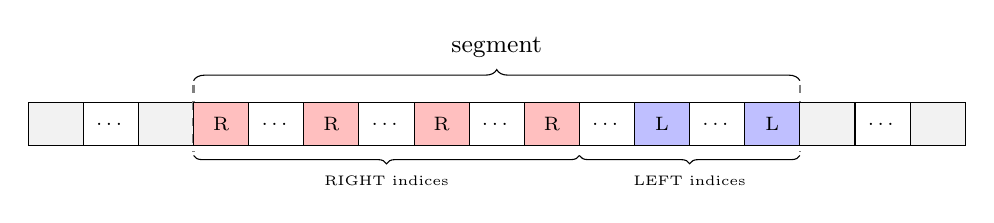
\begin{tikzpicture}[
    cell/.style={minimum width=0.7cm, minimum height=0.55cm, draw, font=\scriptsize},
    dotcell/.style={cell, fill=white},
    right/.style={cell, fill=red!25},
    left/.style={cell, fill=blue!25},
    clean/.style={cell, fill=gray!10},
    boundary/.style={dashed, thick, black!50}
]
% Clean elements before (attached to segment)
\node[clean] (c0) at (0, 0) {};
\node[dotcell] at (0.7, 0) {\dots};
\node[clean] (c1) at (1.4, 0) {};

% Segment boundary (between c1 and r1)
\draw[boundary] (1.75, 0.5) -- (1.75, -0.35);

% R/M region: R ... M ... R ... M
\node[right] (r1) at (2.1, 0) {R};
\node[dotcell] at (2.8, 0) {\dots};
\node[right] (r2) at (3.5, 0) {R};
\node[dotcell] at (4.2, 0) {\dots};
\node[right] (r3) at (4.9, 0) {R};
\node[dotcell] at (5.6, 0) {\dots};
\node[right] (r4) at (6.3, 0) {R};

% L region: ... L ... L
\node[dotcell] at (7.0, 0) {\dots};
\node[left] (l1) at (7.7, 0) {L};
\node[dotcell] at (8.4, 0) {\dots};
\node[left] (l2) at (9.1, 0) {L};

% Segment boundary (between l2 and c2)
\draw[boundary] (9.45, 0.5) -- (9.45, -0.35);

% Clean elements after (attached to segment)
\node[clean] (c2) at (9.8, 0) {};
\node[dotcell] at (10.5, 0) {\dots};
\node[clean] (c3) at (11.2, 0) {};

% Braces
\draw[decorate, decoration={brace, amplitude=4pt}] 
    (1.75, 0.55) -- (9.45, 0.55) node[midway, above=5pt, font=\small] {segment};
\draw[decorate, decoration={brace, amplitude=3pt, mirror}] 
    (1.75, -0.4) -- (6.65, -0.4) node[midway, below=4pt, font=\tiny] {RIGHT indices};
\draw[decorate, decoration={brace, amplitude=3pt, mirror}] 
    (6.65, -0.4) -- (9.45, -0.4) node[midway, below=4pt, font=\tiny] {LEFT indices};
\end{tikzpicture}
\end{center}

DeltaSort operates in two phases:

\begin{enumerate}
  \item \textbf{Phase 1 (Preparation):} Extract dirty values, sort them, write back to
        dirty positions in index order. This establishes direction segments in the array which
        are disjoint and can be repaired independently.
  \item \textbf{Phase 2 (Repair):} Repair each segment left-to-right, deferring RIGHT indices
        to a stack until the first LEFT index is encountered. Flush and repair the the RIGHT
        indexes in stack in LIFO order. Then repair all LEFT indices left-to-right.
\end{enumerate}

\subsection{Key Insight: Directional segmentation enables localized repair}
\label{sec:insight}

The key insight behind DeltaSort is that pre-sorting dirty values induces a
\emph{directional segmentation} of updates. After Phase~1, dirty indices partition
into disjoint segments of the form $(\textrm{R})^*\textrm{L}^+$.

\begin{lemma}[Movement Confinement]
\label{lem:confinement}
Element movement is bounded within each segment: no element crosses a segment boundary.
\end{lemma}

\begin{proof}
Let $S$ be a segment with RIGHT indices $R_1, \ldots, R_m$ followed by LEFT indices
$L_1, \ldots, L_p$. After Phase~1, dirty values are monotonically ordered by index,
so $A[R_1] < \cdots < A[R_m] < A[L_1] < \cdots < A[L_p]$.

\begin{enumerate}
  \item \emph{RIGHT elements cannot pass the leftmost LEFT.}
        Since $A[R_i] < A[L_1]$ for all $i$.

  \item \emph{LEFT elements cannot pass the rightmost RIGHT.}
        Since $A[R_m] < A[L_j]$ for all $j$.
\end{enumerate}

Since no element exits its segment, segments can be repaired independently.
\end{proof}

\subsection{Detailed Algorithm}

\begin{algorithm}[H]
\caption{DeltaSort}
\label{alg:deltasort}
\begin{algorithmic}[1]
\Require Array $A[0..n-1]$, dirty indices $D$, comparator $\texttt{cmp}$
\Ensure $A$ is sorted
\Statex
\State \textbf{Phase 1: Prepare}
\State $\texttt{dirty} \gets \text{sort}(D)$ \Comment{Sort indices ascending}
\State $\texttt{values} \gets [A[d] : d \in \texttt{dirty}]$
\State $\texttt{values} \gets \text{sort}(\texttt{values}, \texttt{cmp})$
\For{$i \gets 0$ \textbf{to} $|\texttt{dirty}| - 1$}
    \State $A[\texttt{dirty}[i]] \gets \texttt{values}[i]$
\EndFor
\Statex
\State \textbf{Phase 2: Repair}
\State $\texttt{pending} \gets []$; $\texttt{leftBound} \gets 0$
\For{$p \gets 0$ \textbf{to} $|\texttt{dirty}| - 1$}
    \State $i \gets \texttt{dirty}[p]$
    \If{$\Call{IsLeftViolation}{A, i}$}
        \State \Call{FlushPending}{$\texttt{pending}, i-1$} \Comment{Fix pending before LEFT}
        \State $\texttt{leftBound} \gets \Call{FixLeftViolation}{A, i, \texttt{leftBound}} + 1$
    \Else
        \State $\texttt{pending.push}(i)$ \Comment{Defer RIGHT indices}
    \EndIf
\EndFor
\Statex
\State \Call{FlushPending}{$\texttt{pending}, n-1$} \Comment{Fix remaining RIGHT violations}
\end{algorithmic}
\end{algorithm}

\vspace{0.5em}

\noindent\begin{minipage}{\linewidth}
\begin{algorithmic}[1]
\Function{IsLeftViolation}{$A$, $i$}
    \State \Return $i > 0 \land \texttt{cmp}(A[i-1], A[i]) > 0$
\EndFunction
\Statex
\Function{IsRightViolation}{$A$, $i$}
    \State \Return $i < n-1 \land \texttt{cmp}(A[i], A[i+1]) > 0$
\EndFunction
\end{algorithmic}
\end{minipage}

\vspace{0.5em}

\noindent\begin{minipage}{\linewidth}
\begin{algorithmic}[1]
\Function{FixLeftViolation}{$A$, $i$, $\texttt{leftBound}$}
    \State $t \gets \Call{BinarySearchLeft}{A, A[i], \texttt{leftBound}, i-1}$
    \State \Call{Move}{A, i, t}
    \State \Return $t$
\EndFunction
\end{algorithmic}
\end{minipage}

\vspace{0.5em}

\noindent\begin{minipage}{\linewidth}
\begin{algorithmic}[1]
\Function{FlushPending}{$\texttt{pending}$, $\texttt{rightBound}$}
    \While{$\texttt{pending} \neq \emptyset$}
        \State $s \gets \texttt{pending.pop}()$ \Comment{Process in LIFO order}
        \If{$\Call{IsRightViolation}{A, s}$}
            \State $t \gets \Call{BinarySearchRight}{A, A[s], s+1, \texttt{rightBound}}$
            \State \Call{Move}{A, s, t}
        \EndIf
    \EndWhile
\EndFunction
\end{algorithmic}
\end{minipage}

\vspace{0.5em}

\noindent\begin{minipage}{\linewidth}
\begin{algorithmic}[1]
\Function{Move}{$A$, $from$, $to$}
    \State $v \gets A[from]$
    \If{$from < to$}
        \State Shift $A[from+1..to]$ left by one
    \ElsIf{$from > to$}
        \State Shift $A[to..from-1]$ right by one
    \EndIf
    \State $A[to] \gets v$
\EndFunction
\end{algorithmic}
\end{minipage}


\subsection{Correctness Proof}

\begin{lemma}[Segment Boundary Invariant]
\label{lem:boundary-invariant}
Segment boundaries are never violated. For any two consecutive segments $S_i$ and 
$S_{i+1}$, all values in $S_i$ remain less than all values in $S_{i+1}$ throughout 
the repair process.
\end{lemma}

\begin{proof}[Proof sketch]
After Phase~1, dirty values are monotonically ordered by index. A segment boundary 
occurs where a LEFT dirty index is followed by a RIGHT dirty index. At such a 
boundary, the RIGHT element satisfies $A[d_{i+1}] \geq A[d_{i+1}-1]$, establishing 
sorted order. By Lemma~\ref{lem:confinement}, movement is confined within segments, 
so boundaries remain intact. A fully rigorous proof is deferred to future work.
\end{proof}

\begin{lemma}[Fixing Does Not Introduce Violations]
\label{lem:fix-invariant}
When a LEFT or RIGHT element is moved to its correct position via binary search, 
no new violations are introduced.
\end{lemma}

\begin{proof}
\emph{LEFT fix}: Binary search finds position $t < i$ where the element belongs. 
Elements in $A[t..i-1]$ shift right by one. The shift preserves relative order. 
By binary search, the moved element satisfies $A[t-1] \leq A[t] < A[t+1]$.

\emph{RIGHT fix}: Binary search finds position $t > s$ where the element belongs. 
Elements in $A[s+1..t]$ shift left by one. The shift preserves relative order. 
By binary search, the moved element satisfies $A[t-1] < A[t] \leq A[t+1]$.

In both cases, no new violations are introduced.
\end{proof}

\begin{theorem}[Correctness]
\label{thm:correctness}
DeltaSort produces a correctly sorted array.
\end{theorem}

\begin{proof}
Phase~2 processes each dirty index exactly once, fixing its violation if any. 
By Lemma~\ref{lem:fix-invariant}, each fix resolves a violation without 
introducing new ones. After all dirty indices are processed, each segment 
is internally sorted.

By Lemma~\ref{lem:boundary-invariant}, segment boundaries maintain sorted 
order throughout. Since each segment is internally sorted and boundaries 
preserve global order, the entire array is sorted.
\end{proof}

\subsection{Algorithm Analysis}

\begin{theorem}[Time Complexity]
\label{thm:time}
DeltaSort runs in $O(k \log k + k \log n + M)$ time, where $M$ is total movement.
\end{theorem}

\begin{proof}
\textbf{Phase 1}: Sort $k$ indices: $O(k \log k)$. Sort $k$ values: $O(k \log k)$.
Write back: $O(k)$.

\textbf{Phase 2}: Each dirty index: $O(1)$ direction check, $O(\log n)$ binary search.
Total: $O(k \log n)$. Movement: $O(M)$.
\end{proof}

\begin{theorem}[Space Complexity]
\label{thm:space}
DeltaSort uses $O(k)$ auxiliary space.
\end{theorem}

\begin{theorem}[Comparison Optimality]
\label{thm:optimal-comparisons}
DeltaSort achieves $O(k \log n)$ comparisons, which matches the information-theoretic
lower bound: each of $k$ dirty elements can occupy any of $n$ final positions, requiring
$\log_2(n^k) = k \log n$ comparisons to distinguish all configurations.
\end{theorem}

\begin{remark}[Movement Efficiency]
While worst-case movement is $O(kn)$, the segmentation created by Phase 1 tends to
reduce movement in practice. When dirty values would otherwise ``cross'' (one moving left,
another right over the same positions), Phase 1 reassigns them to minimize displacement.
Empirical results in \S\ref{sec:experiments} demonstrate substantial speedups, validating
that movement is typically much less than the worst case.
\end{remark}

\begin{table}[h]
\centering
\caption{Algorithm complexity comparison.}
\label{tab:complexity}
\begin{tabular}{l c c c c}
\toprule
Algorithm & Comparisons & Movement & Space & Bounded Search? \\
\midrule
Native Sort & $O(n \log n)$ & $O(n \log n)$ & $O(n)$ & N/A \\
Binary Insertion & $O(k \log n)$ & $O(kn)$ & $O(1)$ & No \\
Extract-Sort-Merge & $O(k \log k + n)$ & $O(n)$ & $O(n)$ & N/A \\
\textbf{DeltaSort} & $O(k \log n)$ & $O(kn)$* & $O(k)$ & Yes \\
\bottomrule
\end{tabular}

\vspace{0.3em}
{\small *Worst case; typically $O(k \cdot \bar{m})$ for average movement distance $\bar{m}$.}
\end{table}

%==============================================================================
\section{Experimental Evaluation}
\label{sec:experiments}
%==============================================================================

\subsection{Baseline Algorithms}

\paragraph{Native Sort.}
Re-sort the entire array: $O(n \log n)$ comparisons, $O(n \log n)$ movements.

\paragraph{Binary Insertion (BI).}
For each $d \in D$: extract all dirty values, then for each: binary search for correct
position, reinsert. Cost: $O(k \log n)$ comparisons, $O(kn)$ worst-case movement.
Always correct, but searches the full array range for each insertion.

\paragraph{Extract-Sort-Merge (ESM).}
Extract dirty values, sort them, merge with clean elements.
Cost: $O(k \log k + n)$ comparisons, $O(n)$ movement.
Always correct but requires $O(n)$ auxiliary space.

\subsection{Setup}

\paragraph{Primary Implementation.} Rust 1.75 (release build with optimizations).

\paragraph{Hardware.} Apple M2 Pro, 16GB RAM, macOS 14.

\paragraph{Algorithms.}
\begin{itemize}
  \item \textbf{Native}: Rust's \texttt{sort\_by} (pattern-defeating quicksort)
  \item \textbf{BI}: Binary Insertion (extract-then-insert)
  \item \textbf{ESM}: Extract-Sort-Merge
  \item \textbf{DS}: DeltaSort
\end{itemize}

\paragraph{Data.} User objects with composite key (country, age, name).
Array sizes $n \in \{1\text{K}, 10\text{K}, 50\text{K}, 100\text{K}, 500\text{K}, 1\text{M}\}$.
Dirty counts $k \in \{1, 5, 10, 20, 50, 100, 200, 500, 1000, 2000, 5000, 10000, 20000\}$.
100 iterations per configuration with 95\% confidence intervals reported.

\subsection{Results}

Table~\ref{tab:rust-results} shows timing results for $n = 50,000$ elements.
DeltaSort consistently outperforms all alternatives up to approximately $k = 10,000$
(20\% of array size), achieving speedups of 7--17$\times$ over Native sort in the
sweet spot ($20 \leq k \leq 200$).

\begin{table}[t]
\centering
\caption{Execution time (\textmu s) for $n = 50,000$ elements. DS vs Best shows speedup
against the fastest alternative (Native, BI, or ESM).}
\label{tab:rust-results}
\begin{tabular}{r r r r r l}
\toprule
$k$ & Native & BI & ESM & DeltaSort & DS vs Best \\
\midrule
1     & 439 & 40 & 188 & \textbf{1} & 62$\times$ faster \\
5     & 749 & 217 & 293 & \textbf{27} & 8$\times$ faster \\
10    & 747 & 525 & 494 & \textbf{44} & 11$\times$ faster \\
20    & 962 & 782 & 655 & \textbf{49} & 13$\times$ faster \\
50    & 1,350 & 1,994 & 1,307 & \textbf{98} & 13$\times$ faster \\
100   & 1,867 & 4,818 & 2,673 & \textbf{109} & 17$\times$ faster \\
200   & 2,560 & 9,022 & 4,785 & \textbf{178} & 14$\times$ faster \\
500   & 3,703 & 22,112 & 11,655 & \textbf{782} & 5$\times$ faster \\
1,000  & 4,253 & 44,481 & 22,480 & \textbf{465} & 9$\times$ faster \\
2,000  & 4,158 & 87,827 & 43,627 & \textbf{837} & 5$\times$ faster \\
5,000  & 4,223 & 211,016 & 102,198 & \textbf{1,751} & 2.4$\times$ faster \\
10,000 & 4,539 & 377,981 & 176,373 & \textbf{3,326} & 1.4$\times$ faster \\
20,000 & \textbf{5,042} & 615,645 & 259,835 & 6,914 & 1.4$\times$ slower \\
\bottomrule
\end{tabular}
\end{table}

Figure~\ref{fig:crossover} visualizes the crossover between DeltaSort and Native sort
on a linear scale. The crossover occurs at $k \approx 13,700$ (27\% of array size),
clearly showing the region where DeltaSort provides substantial speedups.

% Figure: DeltaSort vs Native Sort crossover
\begin{figure}[t]
\centering
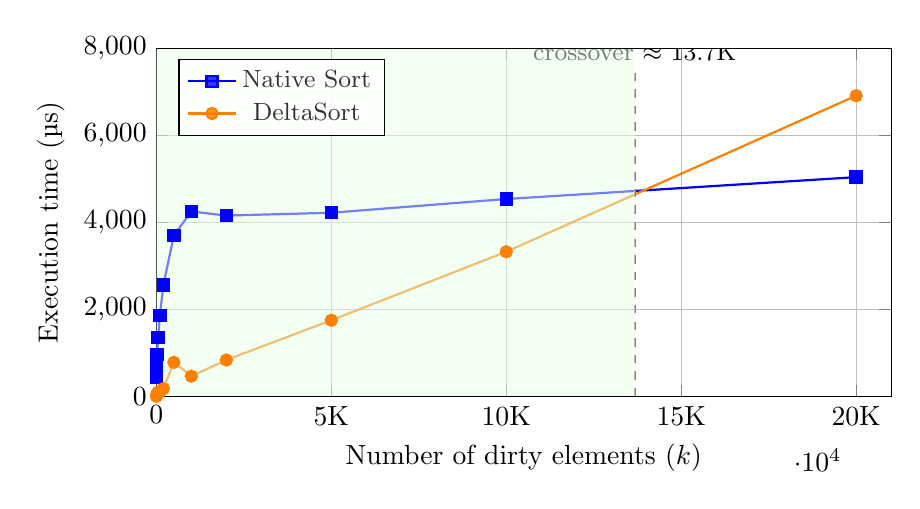
\begin{tikzpicture}
\begin{axis}[
    width=0.9\textwidth,
    height=6cm,
    xlabel={Number of dirty elements ($k$)},
    ylabel={Execution time (\textmu s)},
    xmin=0, xmax=21000,
    ymin=0, ymax=8000,
    xtick={0, 5000, 10000, 15000, 20000},
    xticklabels={0, 5K, 10K, 15K, 20K},
    ytick={0, 2000, 4000, 6000, 8000},
    legend pos=north west,
    legend style={font=\small, fill=white, fill opacity=0.8},
    grid=both,
    grid style={line width=0.1pt, draw=gray!30},
    major grid style={line width=0.2pt, draw=gray!50},
]

% Native sort (relatively flat ~4000-5000 µs)
\addplot[color=blue, mark=square*, thick, mark size=2pt] coordinates {
    (1, 439) (5, 749) (10, 747) (20, 962) (50, 1350) (100, 1867) 
    (200, 2560) (500, 3703) (1000, 4253) (2000, 4158) 
    (5000, 4223) (10000, 4539) (20000, 5042)
};

% DeltaSort (grows linearly with k)
\addplot[color=orange, mark=*, thick, mark size=2pt] coordinates {
    (1, 1) (5, 27) (10, 44) (20, 49) (50, 98) (100, 109) 
    (200, 178) (500, 782) (1000, 465) (2000, 837) 
    (5000, 1751) (10000, 3326) (20000, 6914)
};

% Crossover region annotation
\draw[dashed, thick, gray] (axis cs:13672,0) -- (axis cs:13672,7500);
\node[anchor=south, font=\small] at (axis cs:13672,7500) {crossover $\approx$ 13.7K};

% Shade the "DeltaSort wins" region
\fill[green!10, opacity=0.5] (axis cs:0,0) rectangle (axis cs:13672,8000);

\legend{Native Sort, DeltaSort}
\end{axis}
\end{tikzpicture}
\caption{DeltaSort vs.\ Native Sort for $n = 50,000$. The crossover point occurs at 
$k \approx 13,700$ (27\% of $n$). The shaded region indicates where DeltaSort is faster.}
\label{fig:crossover}
\end{figure}


Figure~\ref{fig:all-algorithms} compares all four algorithms on a log-log scale,
revealing the orders-of-magnitude performance gap between DeltaSort and the baseline
algorithms (BI and ESM) across the full range of $k$ values.

% Figure: All algorithms comparison (log-log scale)
\begin{figure}[H]
\centering
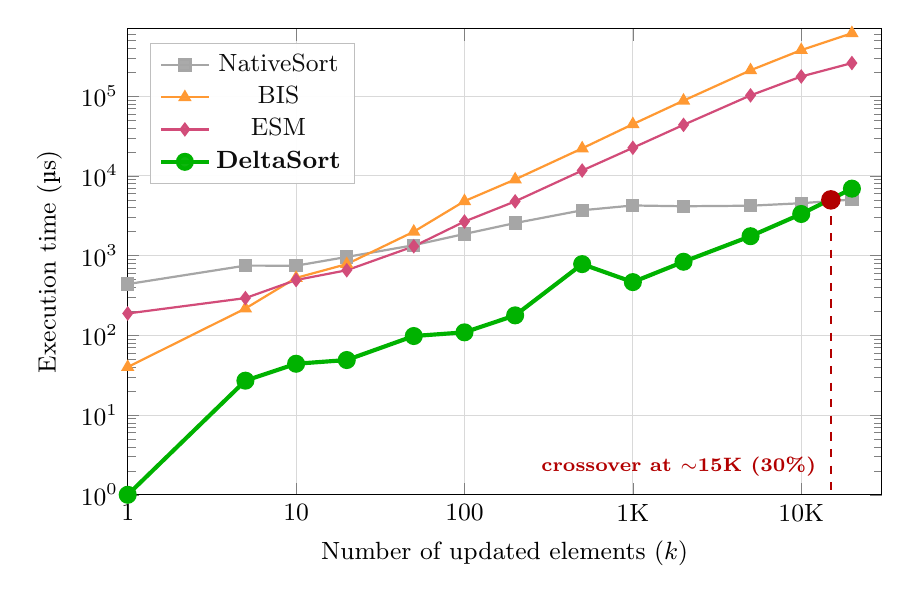
\begin{tikzpicture}
\begin{axis}[
    width=0.92\textwidth,
    height=7.5cm,
    xlabel={Number of updated elements ($k$)},
    ylabel={Execution time (\textmu s)},
    xmode=log,
    ymode=log,
    log basis x=10,
    log basis y=10,
    xmin=1, xmax=30000,
    ymin=1, ymax=700000,
    xtick={1, 10, 100, 1000, 10000},
    xticklabels={1, 10, 100, 1K, 10K},
    legend pos=north west,
    legend style={font=\small, fill=white, fill opacity=0.95, draw=gray!50},
    grid=major,
    major grid style={line width=0.3pt, draw=gray!30},
    tick label style={font=\small},
    label style={font=\small},
]

% NativeSort (horizontal-ish baseline)
\addplot[color=gray!70, mark=square*, thick, mark size=2pt] coordinates {
    (1, 439) (5, 749) (10, 747) (20, 962) (50, 1350) (100, 1867) 
    (200, 2560) (500, 3703) (1000, 4253) (2000, 4158) 
    (5000, 4223) (10000, 4539) (20000, 5042)
};

% Binary Insertion (steep slope)
\addplot[color=orange!80, mark=triangle*, thick, mark size=2pt] coordinates {
    (1, 40) (5, 217) (10, 525) (20, 782) (50, 1994) (100, 4818) 
    (200, 9022) (500, 22112) (1000, 44481) (2000, 87827) 
    (5000, 211016) (10000, 377981) (20000, 615645)
};

% Extract-Sort-Merge
\addplot[color=purple!70, mark=diamond*, thick, mark size=2pt] coordinates {
    (1, 188) (5, 293) (10, 494) (20, 655) (50, 1307) (100, 2673) 
    (200, 4785) (500, 11655) (1000, 22480) (2000, 43627) 
    (5000, 102198) (10000, 176373) (20000, 259835)
};

% DeltaSort (our algorithm - emphasized)
\addplot[color=green!70!black, mark=*, thick, mark size=2.5pt, line width=1.5pt] coordinates {
    (1, 1) (5, 27) (10, 44) (20, 49) (50, 98) (100, 109) 
    (200, 178) (500, 782) (1000, 465) (2000, 837) 
    (5000, 1751) (10000, 3326) (20000, 6914)
};

% Crossover point: bold marker + dashed drop line + label
\node[circle, fill=red!70!black, inner sep=2.5pt] at (axis cs:15000, 5000) {};
\draw[red!70!black, thick, dashed] (axis cs:15000, 5000) -- (axis cs:15000, 1);
\node[font=\scriptsize\bfseries, text=red!70!black, anchor=north east] at (axis cs:14000, 4) {crossover at $\sim$15K (30\%)};

\legend{NativeSort, BIS, ESM, \textbf{DeltaSort}}
\end{axis}
\end{tikzpicture}
\caption{Execution time comparison for $n = 50{,}000$ elements (log-log scale). The vertical dashed line marks the crossover point ($k \approx 15$K) where DeltaSort's advantage over NativeSort diminishes. The shaded region indicates where DeltaSort outperforms all alternatives.}
\label{fig:all-algorithms}
\end{figure}


\subsection{Crossover Analysis}

A key practical question is: at what delta size should one switch from DeltaSort to
Native sort? A binary search was conducted for the crossover point $k_c$ across array
sizes from 1K to 1M elements. Table~\ref{tab:crossover} summarizes the results.

\begin{table}[t]
\centering
\caption{Crossover point $k_c$ where Native sort becomes faster than DeltaSort.}
\label{tab:crossover}
\begin{tabular}{r r r}
\toprule
$n$ & $k_c$ & $k_c / n$ \\
\midrule
1,000 & 235 & 23.5\% \\
2,000 & 469 & 23.4\% \\
5,000 & 1,211 & 24.2\% \\
10,000 & 2,813 & 28.1\% \\
20,000 & 5,782 & 28.9\% \\
50,000 & 13,672 & 27.3\% \\
100,000 & 31,251 & 31.3\% \\
200,000 & 54,688 & 27.3\% \\
500,000 & 105,469 & 21.1\% \\
1,000,000 & 156,251 & 15.6\% \\
\bottomrule
\end{tabular}
\end{table}

The crossover ratio $k_c / n$ ranges from approximately 15\% to 31\%, with most values
falling in the 20--30\% range. This suggests a practical rule of thumb:

\begin{quote}
\emph{Use DeltaSort when fewer than $\sim$25\% of elements are dirty; otherwise use Native sort.}
\end{quote}

\subsection{JavaScript Implementation}

DeltaSort was also implemented in TypeScript running on Node.js v20 (V8 engine). While
the implementation passes all correctness tests, the performance results show higher
variance due to JIT compilation behavior, garbage collection pauses, and other
engine-level effects. The JavaScript benchmarks will be refined in a future revision
to provide more stable measurements. The Rust implementation provides the authoritative
performance characterization.

\subsection{Analysis}

\paragraph{DeltaSort vs.\ Binary Insertion.}
DeltaSort dramatically outperforms BI across all tested configurations, with speedups
ranging from 8$\times$ to over 100$\times$. This is because BI's $O(kn)$ extraction and
insertion costs dominate, while DeltaSort's segmentation enables coordinated processing
that avoids redundant movement.

\paragraph{DeltaSort vs.\ ESM.}
DeltaSort also outperforms ESM for all tested $k$ values up to 10,000. ESM's $O(n)$
merge pass becomes competitive only when $k$ is very large, and even then DeltaSort
remains faster in these measurements.

\paragraph{DeltaSort vs.\ Native Sort.}
The crossover with Native sort occurs at approximately 20--30\% dirty elements. Below
this threshold, DeltaSort's $O(k \log n)$ complexity and efficient stack-based processing
provide substantial speedups. Above this threshold, Native sort's highly optimized
$O(n \log n)$ implementation wins.

\paragraph{Algorithm Selection Guide.}
Based on the Rust benchmarks across array sizes from 1K to 1M elements:

\begin{center}
\begin{tabular}{ll}
\toprule
Condition & Recommendation \\
\midrule
$k \leq 5$ & Binary Insertion (skip Phase 1 overhead) \\
$5 < k < 0.25n$ & \textbf{DeltaSort} \\
$k \geq 0.25n$ & Native Sort \\
\bottomrule
\end{tabular}
\end{center}

\FloatBarrier
%==============================================================================
\section{Future Work}
\label{sec:future}
%==============================================================================

\paragraph{Formal Movement Bounds.}
A conjecture is that Phase 1's segmentation property reduces total element displacement
compared to uncoordinated binary insertion. A formal proof characterizing the expected
movement reduction---potentially in terms of the ``inversion distance'' between original
dirty values and their indices---would strengthen the theoretical foundation.

\paragraph{Cache-Aware Analysis.}
Formalize why bounded search ranges and localized segment processing help despite
unchanged asymptotic complexity.

\paragraph{Block Storage.}
Analyze DeltaSort for B-tree maintenance, where batched updates may reduce node splits.

\paragraph{JavaScript Implementation Refinement.}
The TypeScript/Node.js implementation shows higher variance due to JIT compilation,
garbage collection, and engine-level effects. Future work will characterize and minimize
these effects to provide stable JavaScript benchmarks.

\paragraph{Adaptive Hybrid.}
Runtime selection between DeltaSort and Native sort based on the 25\% crossover threshold,
potentially with dynamic adjustment based on observed performance.

%==============================================================================
\section{Conclusion}
\label{sec:conclusion}
%==============================================================================

This paper presented DeltaSort, a coordinated incremental repair algorithm for sorted arrays.
The key insight is that a pre-sorting phase creates \emph{directional segments}---contiguous
groups of dirty elements that all need to move in the same direction---which can then be
processed efficiently via stack-based coordination.

The main contributions are:

\begin{enumerate}
  \item \textbf{Segmentation via pre-sorting}: Establishing monotonicity among dirty values
        creates directional segments that enable coordinated processing.
  \item \textbf{Stack-based coordination}: LEFT segments are processed immediately with
        progressive search narrowing; RIGHT segments are deferred to a stack and processed
        in LIFO order, ensuring stable target positions.
  \item \textbf{Optimal comparisons}: $O(k \log n)$, matching the information-theoretic
        lower bound.
  \item \textbf{Substantial practical speedup}: 5--17$\times$ over native sort for delta
        sizes up to $\sim$25\% of array size, validated through Rust benchmarks across
        array sizes from 1K to 1M elements.
\end{enumerate}

The crossover point where native sort becomes faster occurs at approximately 25\% dirty
elements, providing a clear decision boundary for practitioners.

The broader lesson is that exploiting application-level knowledge (which indices changed)
enables coordination that blind algorithms cannot achieve. DeltaSort demonstrates that
careful coordination---segmentation plus stack-based processing---yields substantial
practical gains.

%==============================================================================
\bibliographystyle{plain}
\bibliography{refs}
\nocite{*}
\end{document}
